\documentclass{article}

% tight measures:
% \usepackage[margin=0mm, paperwidth=90.7mm, paperheight=126.2mm]{geometry}
% loose measures:
\usepackage[margin=2mm, paperwidth=94.7mm, paperheight=130.2mm]{geometry}

\usepackage{amsmath}
\usepackage{tikz}
\usetikzlibrary{bayesnet}
\usepackage{bm}
\providecommand{\mathbold}[1]{\bm{#1}}
\newcommand{\vct}[1]{\mathbold{#1}}

\begin{document}
\thispagestyle{empty}

\begin{center}
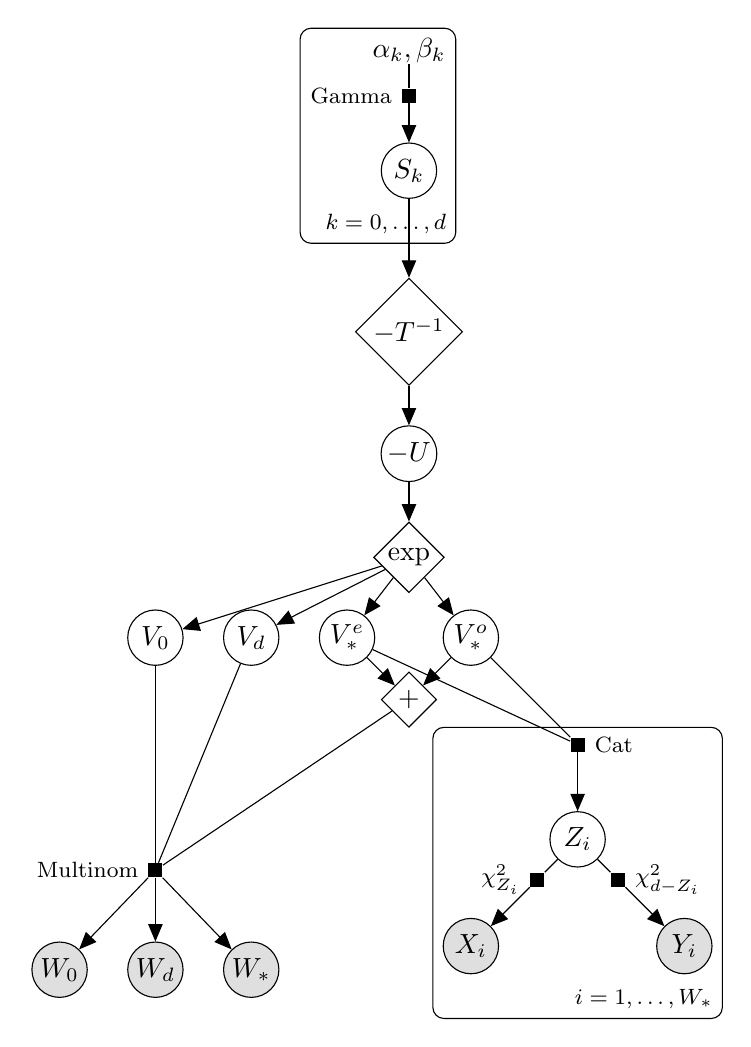
\begin{tikzpicture}
   \node[latent] (vd) {$V_d$} ;
   \node[latent, left=.5 of vd] (v0) {$V_0$} ;
   \node[latent, right=.5 of vd] (veven) {$V^e_*$} ;
 
   \node[det, below right=.5 of veven] (sum) {$+$} ;
   
   \node[latent, above right=.5 of sum] (vodd) {$V^o_*$} ;
 
   \node[latent, above=6 of sum] (t) {$S_k$} ;
   \node[const, above=1 of t] (alpbet) {$\alpha_k,\beta_k$} ;
   \factor[above=.5 of t] {alpbet-t} {left:Gamma} {alpbet} {t} ;
   \plate {alpbett} {(alpbet)(t)} {\rule{2mm}{0mm}$k=0,\ldots,d$} ;   
   \node[det, below=1 of t] (Tinv) {$-T^{-1}$} ;
   \node[latent, below=.5 of Tinv] (u) {$-U$} ;
   \node[det, below=.5 of u] (exp) {$\exp$} ;

   \edge[->] {t} {Tinv} ;
   \edge[->] {Tinv} {u} ;
   \edge[->] {u} {exp} ;
   \edge[->] {exp} {v0,vd,veven,vodd} ;

   \edge[->] {veven,vodd} {sum} ;
   
   \node[obs, below=3.5 of v0] (pd) {$W_d$} ;
   \node[obs, left=.5 of pd] (p0) {$W_0$} ;
   \node[obs, right=.5 of pd] (bulk) {$W_*$} ;
   \factor[below=2.5 of v0] {extr-f} {left:Multinom} {v0,sum,vd} {bulk,p0,pd} ;
   
   \node[obs, below=3.2 of vodd] (X) {$X_i$} ;
   \node[latent, above right=1.2 of X] (K) {$Z_i$} ;
   \node[obs, below right=1.2 of K] (Y) {$Y_i$} ;
   \factor[above right=.7 of X] {X-f} {left:$\chi_{Z_i}^2$} {K} {X} ;
   \factor[above left=.7 of Y] {Y-f} {right:$\chi_{d-Z_i}^2$} {K} {Y} ;
   \factor[above=.75 of K] {K-f} {right:Cat} {veven,vodd} {K} ;

   \plate {KXY} {(K)(K-f)(X)(Y)} {$i=1,\ldots,W_*$} ;
\end{tikzpicture}
\end{center}

\end{document}











